\input{configuration}

\title{Lecture 28 --- Log-Structured File Systems and File Consistency }

\author{Jeff Zarnett \\ \small \texttt{jzarnett@uwaterloo.ca}}
\institute{Department of Electrical and Computer Engineering \\
  University of Waterloo}
\date{\today}


\begin{document}

\begin{frame}
  \titlepage

 \end{frame}


\begin{frame}
\frametitle{Log-Structured File Systems}

The key idea behind a log-structured file system: make all writes sequential.

 For reads, this is not possible, because any data could be requested at any time.\\
 \quad But for writes, that's within our control. 

\end{frame}


\begin{frame}
\frametitle{Log-Structured File Systems}

Both HDD and SSD data storage benefit from this. 

HDD: Minimize seek time.

SSD: Avoid attempting to overwrite in-place.

\end{frame}


\begin{frame}
\frametitle{Log-Structured File Systems}

This idea was proposed in 1992!

The plan, at a high level, is to write data and metadata into buffers of a given size.

When that buffer is full, write it to disk in one sequential write to a big-enough free area.


\end{frame}


\begin{frame}
\frametitle{Finding It Again}

How will we find things again in the future? 

The file itself can be moving, after all, as we write more data to it. 

There must exist some sort of mapping, which is called the \alert{inode map} that is kept up to date.

Yes, but finding the map starts to become a problem.

\end{frame}


\begin{frame}
\frametitle{Finding the Map}

The solution is called the \alert{checkpoint region} -- a clearly-noted fixed location on disk that is the location of the pointers to the latest pieces of the inode map.

That's the way to find everything else.

As you can imagine, this must also contain information on what's free alongside what is allocated.

\end{frame}


\begin{frame}
\frametitle{Writing Sequentially}

Writing sequentially, we know, sort of makes no sense in the SSD world because any write location is as good as any other. 

The main benefit of such a system is that this strategy is already designed for the no-overwrite logic.

The TRIM command can be used to indicate what's reached its time to die. 

\end{frame}


\begin{frame}
\frametitle{Writing Sequentially}

Writing sequentially is the kind of thing that benefits from a certain economy of scale on HDDs.

If we had multiple blocks to go together, we'd write $A, A+1, A+2, A+3...$ in one shot and we'd avoid both seek and rotational latency penalties for 3 of the 4.

In the limit, we could amortize rotational latency to be negligible.

\end{frame}


\begin{frame}
\frametitle{Writing Sequentially}

Okay, infinite write size is not possible and we've identified that a buffer size of 1 block doesn't meet our goals either because the intention is to amortize the cost. 

\begin{center}
	
\includegraphics[width=0.4\textwidth]{images/narrows.png}
\end{center}

Having narrowed it down to somewhere between 1 and infinity is not helpful.


\end{frame}


\begin{frame}
\frametitle{Set a Target}

If we target, let's say, 90\% of the maximum effective rate, that allows setting the buffer size to a specific number. 

There's nothing magical about 90\% as a target -- but it is reasonable enough. 

\begin{center}
$D = \dfrac{F}{1-F} \times R_{peak} \times T_{position}$
\end{center}

\end{frame}



\begin{frame}
\frametitle{New Problem}

We introduced a new problem, here. 

If the system crashes (or loses power) when we have a large buffer that's mostly full, we could lose a lot of progress.  

We know that this could happen at any time. LFS addresses this by being prepared for such an eventuality and having a \alert{recovery strategy}. 

A recovery strategy is exactly what it sounds like, a way to get things back to a consistent state.

\end{frame}


\begin{frame}
\frametitle{Recovery Strategy}

Let's zoom out for a bit and take a look at a specific kind of recovery for file systems.

\end{frame}


\begin{frame}
\frametitle{Consistency Checking and Journalling}

Unfortunately, an error, crash, or power failure or something similar may result in a loss of data or inconsistent data in the file system. 

The directory structures, pointers, inodes, FCBs, et cetera are all data structures and if they become corrupted it may lead to serious problems.


\end{frame}

\begin{frame}
\frametitle{Consistency Checking}

We could check for inconsistent data periodically (e.g., on system boot up) and many operating systems do so. 

This is, of course, an operation that will consume a very large amount of time while the whole disk is scanned. 

UNIX: \texttt{fsck}. Windows: \texttt{chkdsk}/\texttt{scandisk}.

\begin{center}
	
\includegraphics[width=0.3\textwidth]{images/swearwords.jpg}
\end{center}

\end{frame}

\begin{frame}
\frametitle{Consistency Checking}

These tools will look for inconsistent states (e.g., a file that claims to be 12 blocks but the linked list contains only 5) and will attempt to repair it.

Its level of success depends on the nature of the problem and the implementation of the file system.

\end{frame}



\begin{frame}
\frametitle{Preventing the Problem}

Obviously we would like to prevent the problem, if we can. 

Atomic operations: an operation should either succeed completely, or not take place at all. 

This approach is used in the Windows NTFS system as well as Mac OS HFS+.


\end{frame}

\begin{frame}
\frametitle{Transactions}

We might be familiar, at this point, with the concept of the \alert{transaction}.

Before making any changes, make a list of all the things we plan to do. 

Then do the things written down. 

Then we consider the transaction complete.

\end{frame}

\begin{frame}
\frametitle{Transactions}

All metadata changes are written sequentially to a log file; once the changes are written to the log, control returns to the program that requested the operation. 

Meanwhile, the log entries are actually carried out. 

As changes are made, a pointer is updated to indicate which of the log entries have really happened and which have not.

When an entire transaction is completed, it is removed from the log file. If the system crashes, the log file will contain zero or more transactions.
\end{frame}

\begin{frame}
\frametitle{Transactions}

If zero, there is no problem: nothing was in progress at the time of the crash. 

If there are some, then the transactions were not completed and the operations should still be carried out. 

If a transaction was aborted (not committed), we walk backwards through the log entries to undo any completed operations.

Thus, we go back to the state before the start of the transaction.




\end{frame}

\begin{frame}
\frametitle{Data Loss}

Even though a particular write may not have taken place because of a crash, resulting in some data loss, the system will always remain in a consistent state. 

As a side benefit, we can sometimes re-order the writes to get better performance (e.g., schedule them to get better disk utilization). 


\end{frame}

\begin{frame}
\frametitle{ZFS Approach}

The approach in the Solaris ZFS is similar, but not identical. 

Blocks are never overwritten with new data.\\
\quad Instead, a transaction writes all data and metadata to new blocks. 

Only when the transaction is complete, any references to the old blocks are replaced with the location of the new blocks. 


Then the old pointers and blocks can be cleaned up (reused or disposed of). 


\end{frame}



\begin{frame}
\frametitle{Example: NTFS (Windows File System)}

NTFS uses several different storage levels:

\begin{enumerate}
	\item \textbf{Sector}
	\item \textbf{Cluster}
	\item \textbf{Volume}
\end{enumerate}


\end{frame}

\begin{frame}
\frametitle{NTFS}

The cluster is the fundamental unit of allocation of NTFS.

This allows the file system to be independent of the size of physical sectors on the disk. 

A volume contains file system information, a collection of files, and free space. 

The logical volume may be some of a physical disk, all of one, or spread across multiple physical disks.

\end{frame}

\begin{frame}
\frametitle{NTFS Volume Layout}

\begin{center}
	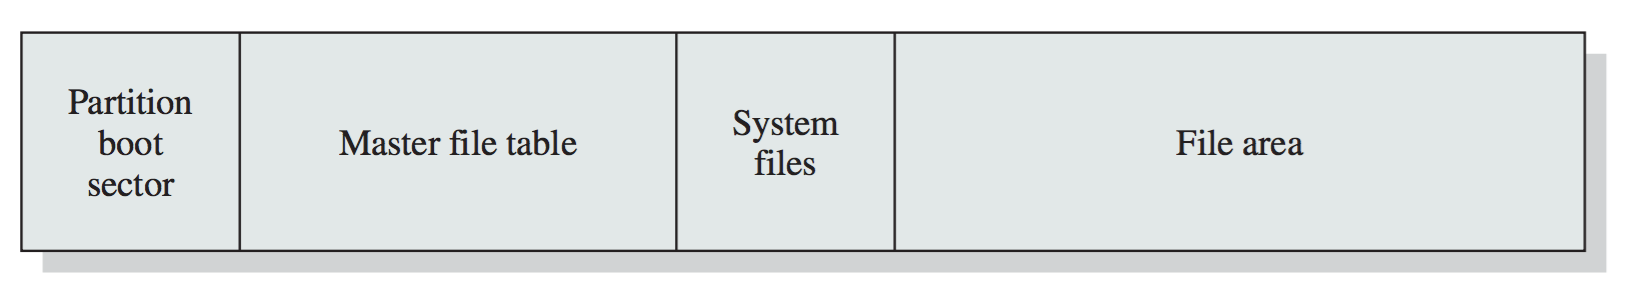
\includegraphics[width=0.9\textwidth]{images/ntfs-volume.png}
\end{center}

\end{frame}

\begin{frame}
\frametitle{NTFS System Files}

The Master File Table (MFT) contains information about all the files and folders. 

A block is allocated to system files that contain important system information:

\begin{enumerate}
	\item \textbf{MFT2}
	\item \textbf{Log File}
	\item \textbf{Cluster Bitmap}
	\item \textbf{Attribute Definition Table}
\end{enumerate}
\end{frame}



\begin{frame}
\frametitle{NTFS File and Directory Attributes}

\begin{center}
	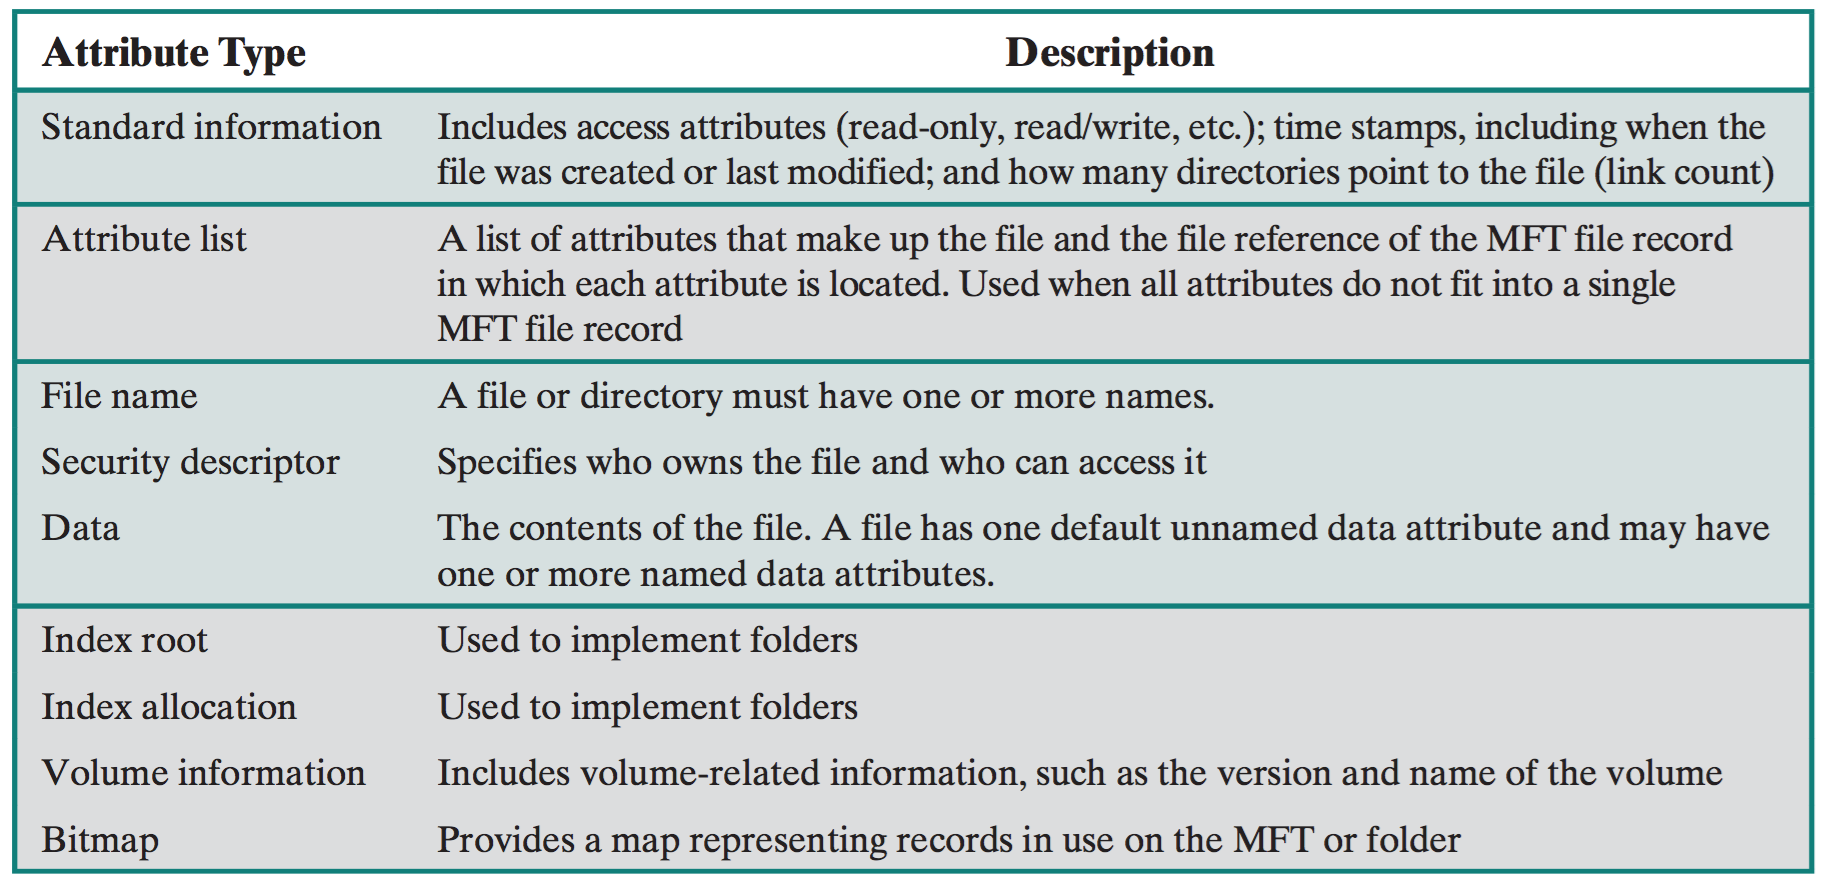
\includegraphics[width=\textwidth]{images/ntfs-attrs.png}
\end{center}


\end{frame}

\begin{frame}
\frametitle{NTFS Journalling}

NTFS uses journalling to ensure that the file system will be in a consistent state at all times, even after a crash or restart. 

There is a service responsible for maintaining a log file that will be used to recover in the event that things go wrong.  

Note that the goal of recovery is to make sure the system-maintained metadata is in a consistent state; user data can still get lost. 

This was a Microsoft design decision.


\end{frame}

\begin{frame}
\frametitle{NTFS Journalling Implementation}

The actual implementation of journalling:

\begin{enumerate}
	\item Record the change(s) in the log file in the cache.
	\item Modify the volume in the cache.
	\item The cache manager flushes the log file to disk.
	\item Only after the log file is flushed to disk, the cache manager flushes the volume changes.
\end{enumerate}

\end{frame}

\begin{frame}
\frametitle{Backups}

We often think of them as places for permanent storage of data, but hard drives can and do fail. 


\begin{center}
	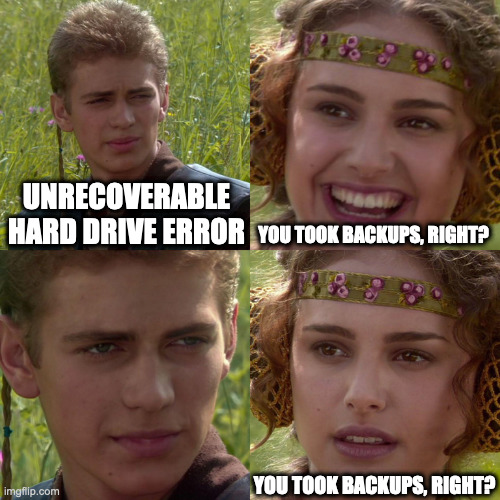
\includegraphics[width=0.5\textwidth]{images/backups.jpg}
\end{center}

So please, take backups of important data.


\end{frame}

\end{document}

